\subsection{Premi::Front-End::Views}
	\subsubsection*{Informazioni sul package}
		\begin{figure}[h]
			\centering
			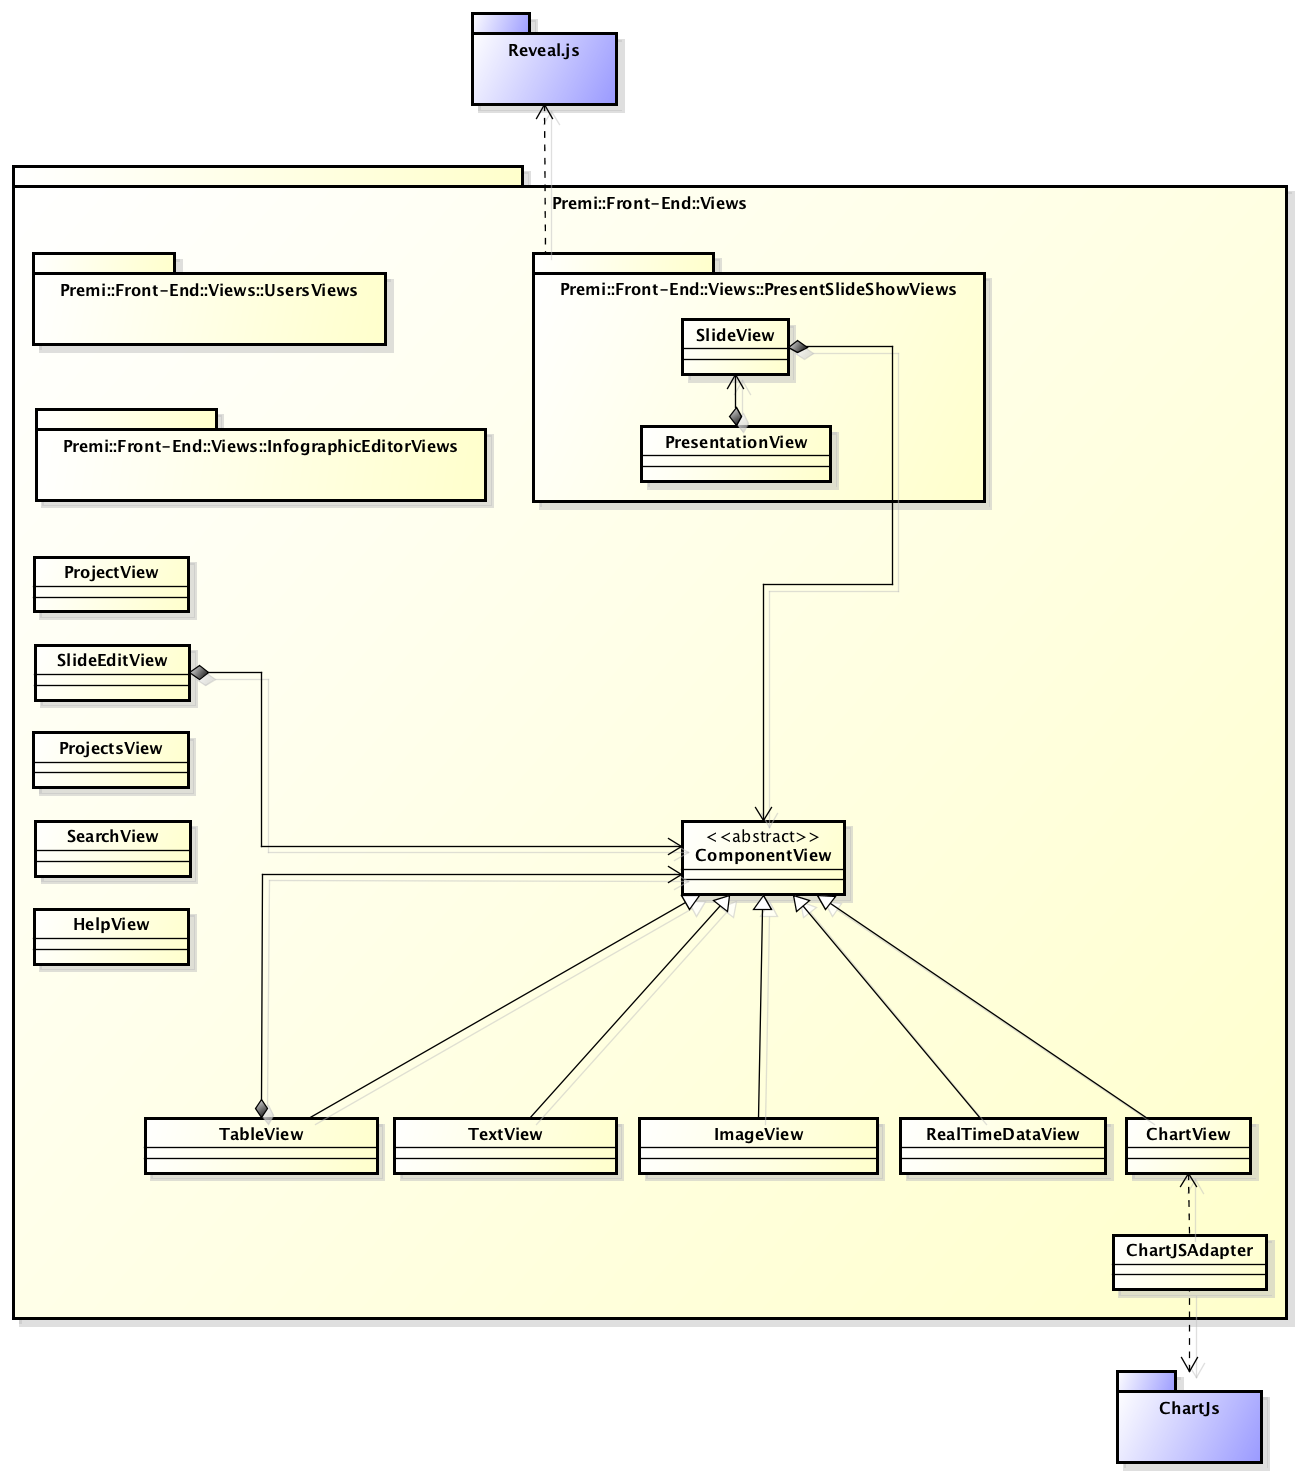
\includegraphics[width=0.7\linewidth]{img/front-end_views}
			\caption[Premi::Front-End::Views]{Premi::Front-End::Views}
		\end{figure}
		Il package contiene gli elementi per creare la parte grafica del front-end, la visualizzazione delle pagine e dell'editor del progetto.

	\subsubsection*{Package contenuti:}

	\begin{itemize}
		\item Premi::Front-End::Views::UsersViews:
			\begin{itemize}
				\item \textbf{Descrizione}: classe per la gestione delle pagine riguardanti l'accesso al sito.
			\end{itemize}

		\item Premi::Front-End::Views::PresentSlideShowViews:
			\begin{itemize}
				\item \textbf{Descrizione}: classe per la gestione delle pagine per la visualizzazione della presentazione.
			\end{itemize}

		\item Premi::Front-End::Views::InfographicsEditorViews:
		\begin{itemize}
			\item \textbf{Descrizione}: classe per la gestione delle infografiche relative al progetto.
		\end{itemize}
	\end{itemize}

	\subsubsection*{Classi contenute:}
	\begin{itemize}

		\item Premi::Front-End::Views::UsersViews:
		\begin{itemize}
			\item \textbf{Descrizione}: classe per la gestione delle pagine riguardanti l'accesso al sito.
		\end{itemize}

		\item Premi::Front-End::Views::ProjectView:
		\begin{itemize}
			\item \textbf{Descrizione}: classe per la gestione della pagina del progetto attualmente aperto dall'utente.
		\end{itemize}

		\item Premi::Front-End::Views::SlideEditView:
		\begin{itemize}
			\item \textbf{Descrizione}: classe per la gestione della pagina dell'editor di una slide;
			\item \textbf{Relazioni con altre classi}:
			\begin{itemize}
				\item Premi::Front-End::Views::ComponentView.
			\end{itemize}
		\end{itemize}

		\item Premi::Front-End::Views::ProjectsView:
		\begin{itemize}
			\item \textbf{Descrizione}: classe per la gestione della pagina contenente i progetti creati da un utente.
		\end{itemize}

		\item Premi::Front-End::Views::SearchView:
		\begin{itemize}
			\item \textbf{Descrizione}: classe per la gestione della pagina per la ricerca di un progetto e la visualizzazione dei risultati.
		\end{itemize}

		\item Premi::Front-End::Views::HelpView:
		\begin{itemize}
			\item \textbf{Descrizione}: classe per la gestione della pagina della guida dell'applicazione.
		\end{itemize}

		\item Premi::Front-End::Views::ComponentView:
		\begin{itemize}
			\item \textbf{Descrizione}: classe base per la gestione grafica degli elementi che è possibile includere in una slide.
		\end{itemize}

		\item Premi::Front-End::Views::TableView:
		\begin{itemize}
			\item \textbf{Descrizione}: classe per la gestione grafica dell'elemento tabella che è possibile includere in una slide. Può essere composta da altri elementi della classe *::ComponentView;
			\item \textbf{Relazioni con altre classi}:
			\begin{itemize}
				\item Premi::Front-End::Views::ComponentView.
			\end{itemize}
		\end{itemize}


		\item Premi::Front-End::Views::TextView:
		\begin{itemize}
			\item \textbf{Descrizione}: classe per la gestione grafica dell'elemento casella di testo che è possibile includere in una slide;
			\item \textbf{Relazioni con altre classi}:
			\begin{itemize}
				\item Premi::Front-End::Views::ComponentView.
			\end{itemize}
		\end{itemize}

		\item Premi::Front-End::Views::ImageView:
		\begin{itemize}
			\item \textbf{Descrizione}: classe per la gestione grafica dell'elemento immagine che è possibile includere in una slide;
			\item \textbf{Relazioni con altre classi}:
			\begin{itemize}
				\item Premi::Front-End::Views::ComponentView.
			\end{itemize}
		\end{itemize}

		\item Premi::Front-End::Views::RealTimeDataView:
		\begin{itemize}
			\item \textbf{Descrizione}: classe per la gestione grafica dell'elemento di dati real-time che è possibile includere in una slide;
			\item \textbf{Relazioni con altre classi}:
			\begin{itemize}
				\item Premi::Front-End::Views::ComponentView.
			\end{itemize}
		\end{itemize}

		\item Premi::Front-End::Views::ChartView:
		\begin{itemize}
			\item \textbf{Descrizione}: classe per la gestione grafica dell'elemento grafico che è possibile includere in una slide;
			\item \textbf{Relazioni con altre classi}:
			\begin{itemize}
				\item Premi::Front-End::Views::ComponentView;
				\item Premi::Front-End::Views::ChartJsAdapter;
			\end{itemize}
		\end{itemize}

		\item Premi::Front-End::Views::ChartJsAdapter:
		\begin{itemize}
			\item \textbf{Descrizione}: classe per interfacciare l'utilizzo della classe Chart.Js con la classe ChartView;
			\item \textbf{Relazioni con altre classi}:
			\begin{itemize}
				\item Premi::Front-End::Views::ChartView;
			\end{itemize}
			\item \textbf{Relazioni con altri package}:
			\begin{itemize}
				\item Chart.Js
			\end{itemize}
		\end{itemize}
	\end{itemize}


\subsection{Premi::Front-End::Views::UsersViews}
	\subsubsection*{Informazioni sul package}
	\begin{figure}[h]
		\centering
		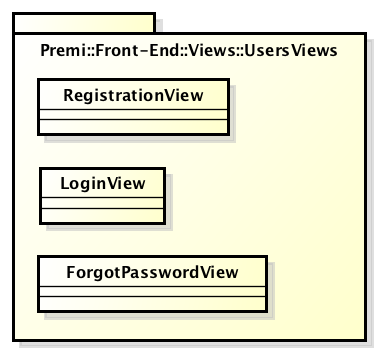
\includegraphics[width=0.7\linewidth]{img/front-end_views_usersviews}
		\caption[Premi::Front-End::Views::UsersViews]{Premi::Front-End::Views::UsersViews}
	\end{figure}
	Il package contiene le classi per creare la parte grafica dell'accesso di un utente all'applicazione.

	\subsubsection*{Classi contenute:}
	\begin{itemize}

		\item Premi::Front-End::Views::UsersViews::RegistrationView:
		\begin{itemize}
			\item \textbf{Descrizione}: classe per creare la sezione relativa alla registrazione di un nuovo utente.
		\end{itemize}

		\item Premi::Front-End::Views::UsersViews::LoginView:
		\begin{itemize}
			\item \textbf{Descrizione}: classe per creare la sezione relativa al login di utente già registrato.
		\end{itemize}

		\item Premi::Front-End::Views::UsersViews::ForgotPasswordView:
		\begin{itemize}
			\item \textbf{Descrizione}: classe per creare la sezione relativa al recupero della password per l'utente registrato.
		\end{itemize}
	\end{itemize}


\subsection{Premi::Front-End::Views::PresentSlideShowViews}
	\subsubsection*{Informazioni sul package}
	\begin{figure}[h]
		\centering
		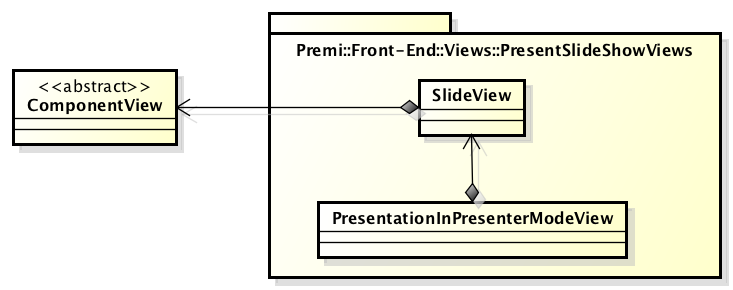
\includegraphics[width=0.7\linewidth]{img/front-end_views_presentslideshowviews}
		\caption[Premi::Front-End::Views::PresentSlideShowViews]{Premi::Front-End::Views::PresentSlideShowViews}
	\end{figure}
	Il package contiene le classi per la parte grafica relativa alla visualizzazione della presentazione da parte dell'utente.

	\subsubsection*{Classi contenute:}
		\begin{itemize}
			\item Premi::Front-End::Views::PresentSlideShowViews::SlideView:
			\begin{itemize}
				\item \textbf{Descrizione}: classe per creare la parte grafica di una slide nella visualizzazione di una presentazione. È composta da oggetti della classe ComponentView,o sue derivate;
				\item \textbf{Relazioni con altre classi}:
				\begin{itemize}
					\item Premi::Front-End::Views::ComponentView.
				\end{itemize}
			\end{itemize}

			\item Premi::Front-End::Views::PresentSlideShowViews::PresentationInPresenterModeView:
			\begin{itemize}
				\item \textbf{Descrizione}: classe per creare la parte grafica di una slide nella visualizzazione di una presentazione nella modalità presentatore. È composta da oggetti della classe SlideView in quanto la contiene implementandola;
				\item \textbf{Relazioni con altre classi}:
				\begin{itemize}
					\item Premi::Front-End::Views::PresentSlideShowViews::SlideView.
				\end{itemize}
			\end{itemize}
		\end{itemize}

\subsection{Premi::Front-End::Views::InfographicEditorViews}
	\subsubsection*{Informazioni sul package}
	\begin{figure}[h]
		\centering
		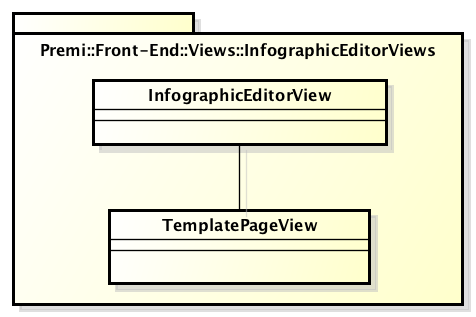
\includegraphics[width=0.7\linewidth]{img/front-end_views_infographiceditorviews}
		\caption[Premi::Front-End::Views::InfographicEditorViews]{Premi::Front-End::Views::InfographicEditorViews}
	\end{figure}
	Il package contiene le classi per la parte grafica relativa alle infografiche e alla loro creazione.

	\subsubsection*{Classi contenute:}
	\begin{itemize}

		\item Premi::Front-End::Views::InfographicEditorViews::InfographicEditorView:
		\begin{itemize}
			\item \textbf{Descrizione}: classe per creare un'infografica. Permette la personalizzazione di essa attraverso la selezione delle slide da usare.
		\end{itemize}

		\item Premi::Front-End::Views::InfographicEditorViews::TemplatePageView:
		\begin{itemize}
			\item \textbf{Descrizione}: classe che permette di creare la sezione per selezionare il template da utilizzare nell'infografica;
			\item \textbf{Relazioni con altre classi}:
			\begin{itemize}
				\item Premi::Front-End::Views::InfographicEditorViews::InfographicEditorView.
			\end{itemize}
		\end{itemize}
	\end{itemize}
